\par Kotlin is a cross-platform, statically typed, general-purpose programming language with type inference. Kotlin is designed to interoperate fully with Java, and the JVM version of Kotlin's standard library depends on the Java Class Library, but type inference allows its syntax to be more concise. Kotlin mainly targets the JVM, but also compiles to JavaScript (e.g. for frontend web applications using React) or native code (via LLVM), e.g. for native iOS apps sharing business logic with Android apps. % wikipedia

\par Kotlin has quickly skyrocketed in popularity. It's used by companies like Google, Square, Pinterest, Pivotal, Netflix and Atlassian. It's the fastest-growing programming language, according to GitHub, growing over 2,5 times in the past year. It was voted one of the five most loved languages, according to Stack Overflow. There are even meetups focused on Kotlin. \footnote{\url{https://www.businessinsider.com/kotlin-programming-language-explained-popularity-2019-5\#:\~:text=Kotlin\%20has\%20quickly\%20skyrocketed\%20in,times\%20in\%20the\%20past\%20year}}
% https://www.businessinsider.com/kotlin-programming-language-explained-popularity-2019-5#:~:text=Kotlin%20has%20quickly%20skyrocketed%20in,times%20in%20the%20past%20year.
\par Kotlin is used in a lot of ways. For example it can be used for backend development using ktor framework (developed by JetBrains), and spring framework also has first-party support for kotlin (Spring is one of the most popular framework on Java for Web development). Kotlin/JS provides the ability to transpile your Kotlin code to JavaScript, as well as providing JS variant of kotlin standard library and interopability with existing JS dependencies, both for Node.js and browser. There are numerous ways that Kotlin/JS can be used. For instance, you can write frontend web applications using Kotlin/JS,
write server-side and serverless applications using Kotlin/JS, create libraries for use with JavaScript and TypeScript. Support for multiplatform programming is one of Kotlin’s key benefits. It reduces time spent writing and maintaining the same code for different platforms while retaining the flexibility and benefits of native programming. 

\par Asynchronous or non-blocking programming is the new reality. Whether we're creating server-side, desktop or mobile applications, it's important that we provide an experience that is not only fluid from the user's perspective, but scalable when needed.
There are many approaches to this problem, and Kotlin takes a very flexible one by providing Coroutine support as a first-party library kotlinx.coroutines with a kotlin compiler plugin and delegating most of the functionality to libraries, much in line with Kotlin's philosophy.
As a bonus, coroutines not only open the doors to asynchronous programming, but also provide a wealth of other possibilities such as concurrency, actors, etc.

A coroutine is a concurrency design pattern that you can use on Android to simplify code that executes asynchronously. Coroutines(in a form of kotlinx.coroutines library and kotlin compiler plugin) were added to Kotlin in version 1.3 and are based on established concepts from other languages.

On Android, coroutines help to manage long-running tasks that might otherwise block the main thread and cause your app to become unresponsive. Over 50\% of professional developers who use coroutines have reported seeing increased productivity. Coroutines enable you to write cleaner and more concise app code.

The state of Kotlin in 2020 (according to the latest Kotlin Census and statistical data)
\begin{itemize}
    \item 4,7 million users
    \item 65\% of users use Kotlin in production
    \item For 56\% of users, Kotlin is their primary language, which means the main or only
    one they use at work
    \item 100+ people are on the Kotlin development team at JetBrains
    \item 350+ independent contributors develop the language and its ecosystem outside
    of JetBrains
\end{itemize}

% https://techcrunch.com/2019/05/07/kotlin-is-now-googles-preferred-language-for-android-app-development/
Kotlin is widely used among Android developers, including open source OS, like HarmonyOS, that are compatible with Android. In 2019 Google announced that the Kotlin programming language is now its preferred language for Android app developers. In the same year Stack Overflow stated that Kotlin is fourth most loved language in community. Nowadays there are over 60\% of android developers who use Kotlin as their main language. \footnote{\url{https://techcrunch.com/2019/05/07/kotlin-is-now-googles-preferred-language-for-android-app-development/}}
\par Kotlin's popularity can be explained by the rising number of Android users (last year, 124.4m in the USA) and, thus, Android-based devices. 80\% of Kotlin programmers use the language to build Android apps, 31\% for back-end applications, 30\% for SDK/libraries.
Kotlin is also interoperable with Java, which allows developers to use all existing Android libraries in a Kotlin app. Kotlin is in the top of PYPL rating.
\newline
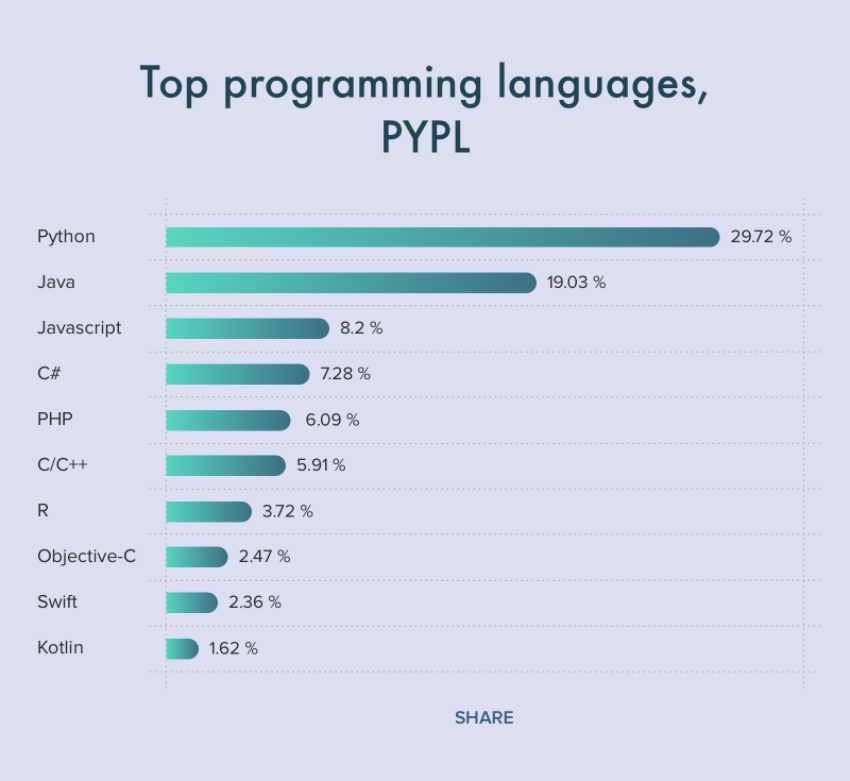
\includegraphics[scale = 0.5]{pictures/kotlinRating.png}
\newline
\par Overall, Kotlin is a modern language that gain it's popularity incredibly fast. It is mostly used by Android developers, but other "branches of programming" are gaining popularity as well, for example spring framework(the most popular Java framework) is supporting Kotlin. It supports both OO (object-oriented) and FP (function-oriented) programming paradigms. Since release 1.4 Kotlin claims to bring major updated every 6 month.